\chapter{Introdução}
\label{cap1}


\section{Fundamentação Teórica}


A fim de orientar o análise encontrada neste trabalho, se faz necessário a descrição e pesquisa por fundamentação teórica dos conceitos básicos relevantes no contexto de microsserviços e implantação dessas arquiteturas.
%
Por esse motivo, esta seção irá introduzir os conceitos de microsserviços, containers, docker e implantação utilizando a técnica de docker swarm.


\subsection{Microserviços}
Entende-se por microsserviço aplicações que executam operações menores de um macrosserviço, da melhor forma possível~\cite{stephenclarkewillson2017, Newman2015Feb}.

Um microsserviço é definido pelas seguintes características~\cite{8169955}:


\begin{itemize}
  \item Deve possibilitar a implementação como uma peça individual do macrosserviço.
  \item Deve funcionar individualmente.
  \item Cada serviço deve ter uma interface. Essa interface deve ser o suficiente para utilizar o microsserviço.
  \item A interface deve estar disponível na rede para chamada de processamento remoto ou consulta de dados.
  \item O serviço pode ser utilizado por qualquer linguagem de programação e/ou plataforma.
  \item O serviço deve executar com as dependências mínimas.
  \item Ao agregar vários microsserviços, o macrosserviço resultante poderá prover funcionalidades complexas.
\end{itemize}



\subsection{Containers}
Os container permitem ao desenvolvedor "empacotar" sua aplicação e todas as suas dependências(ex. bibliotecas), dessa forma, lhe é garantido que a aplicação terá o mesmo comportamento independentemente do hospedeiro Linux.

\subsection{Docker}
Docker é uma plataforma que nos permite "construir, emabarcar e rodar uma aplicação em qualquer lugar". Ele percorreu um longo caminho em um período de tempo incrivelmente curto e atualmente é considerado uma solução padrão para um dos apectos mais custosos do software: a implantação (citar Docker in Pratice)

Docker é uma ferramenta desenvolvida para facilitar o processo de criação, implantação e execução de aplicações por meio do uso de containers.
Pode ser pensado como um tipo de maquina virtual, porém diferentemente desta que necessita a criação de todo um sistema operacional virtual, o Docker, permite que as aplicações compartilhem o mesmo kernel Linux que o hospedeiro, reduzindo assim o tamanho da aplicação e obtendo um ganho de desempenho.

\subsection{Docker Swarm}
É uma ferramenta nativa do Docker que permite criar clusters de containers, chamado swarms, o que possibilitam a escalabilidade de recursos de acordo com a demanda(carga) (citar The Docker Book)
O que possibilita que diversos hospedeiros de Docker estejam inseridos no mesmo pool de recursos, facilitando assim a implantação de containers, uma vez que o Swarm disponibiliza uma API de integração que abstrai grande parte das
atividades necessárias a administração dos conteiners e promove um tipo de tolerancia a falhas
\section{Histórico}

\subsection{Arquitetura Monolítica}
(Pensar ) Arquitetura Monolítica, é uma arquitetura de desenvolvimento, na qual típicamente , apesar da complexidade dos sistemas ser quebrada ao se utilizar módulos, esses são projetados para a criação de um único executável, o qual possui todos os seus módulos executados em um mesma máquina.
Com o passar do tempo, o sistema cresce e tende a tornar-se cada vez mais complexo, o que gera diversos problemas em sua manutenção, por exemplo temos, a escalabilidade do sistema, que exige que o mesmo seja replicado inteiramente, mesmo que apenas uma parte desse seja necessária na nova instância, aumentando assim os custos.

\subsection{Arquitetura de Microsserviços}
\label{sec:microsservicos}
%
O objetivo de uma arquitetura de microsserviços é funcionar separadamente de forma autônoma, contendo baixo acoplamento~\cite{Newman2015Feb}.
%
Seu funcionamento deve ser desenhado para permitir alinhamentos de alta coesão e baixo acoplamento entre os demais microsserviços existentes em um macrosserviço~\cite{8169955}.



Arquiteturas de microsserviços iniciam uma nova linha de desenvolvimento de aplicações preparadas para executar sobre nuvens computacionais, promovendo maior flexibilidade, escalabilidade, gerenciamento e desempenho, sendo a principal escolha de arquitetura de grandes empresas como Amazon, Netflix e LinkedIn~\cite{7830692,7515686}.

\begin{figure}[htb!]
\caption{Microsserviços podem ter diferentes tecnologias}
\label{fig:microsservicos_tecnologias}
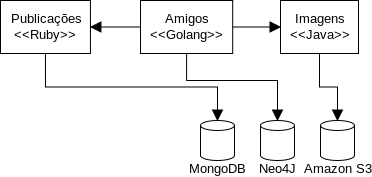
\includegraphics[height=4cm]{img/cap2/microsservicos_tecnologias.png}
\centering

Adaptado de:~\cite{Newman2015Feb}
\end{figure}

O microsserviço deverá ser uma entidade separada. Ela deve ser implantada como um sistema independente em um \ac{paas}.
%
Toda a comunicação entre os microsserviços de um macrosserviço será executada sobre a rede, a fim de reforçar a separação entre cada serviço.
%
As chamadas pela rede com o cliente ou entre os microsserviços será executada através de uma \ac{api}, permitindo a liberdade de tecnologia em que cada um será implementado~\cite{Newman2015Feb}.



\begin{figure}[htb!]
\caption{Microsserviços são escaláveis}
\label{fig:microsservicos_escalabilidade}
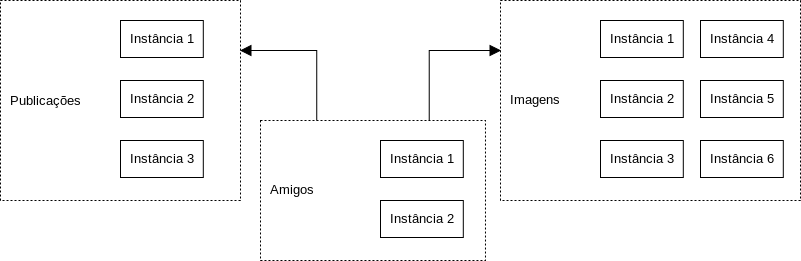
\includegraphics[height=5cm]{img/cap2/microsservicos_escalabilidade.png}
\centering

Adaptado de:~\cite{Newman2015Feb}
\end{figure}



Uma arquitetura de microsserviços é escalável, como visível na Figura \ref{fig:microsservicos_escalabilidade}.
%
Ela permite o aumento do número de microsserviços sob demanda para suprir a necessidade de escalabilidade.
%
Este modelo computacional obtém maior desempenho, principalmente se executar sobre plataformas de computação elástica, na qual o orquestrador do macrosserviço pode aumentar o número de instâncias conforme a necessidade de requisições~\cite{Nadareishvili2016Aug}.


\section{Funcionamento}

\section{Boas práticas}
\begin{itemize}
	\item Não armazenar dados em containers, uma vez que esses podem ser parados, destruidos ou mesmo substituidos, se ncessário armazenar dados deve ser feito em um volume, com o cuidado de evitar que dois ou mais containers escrevam dados em um mesmo volume, o que poderia causar o corrompimento dos dados.
	\item Não criar imagens grandes, já que essas possuirão uma distribuição complexa, uma imagens de possuir apenas as bibliotecas e arquivos necessários para a execução da aplicação ou processo.
	\item Não executar mais de um processo/aplicação em um único container, pois tal comportamento acarretará em aumento da complexidade do gerenciamento e no número de logs.
	\item Não dos endereços IP dos containers, o endereço IP do container pode se alterado quando o mesmo é iniciado e parado. Caso seja necessária a comunicação entre a aplicação ou microsserviço e um outro container, é recomendado o uso de variáveis de ambiente para transmitir o hostname e porta corretos de um container para outro.
\end{itemize}



\section{Principais aplicações}

\subsection{Aplicações Web}

Microsserviços desenvolvidos para web utilizam arquitetura \ac{rest} baseado sobre o protocolo \ac{http}.
É uma boa prática utilizar o corpo com conteúdo da requisição e resposta no formato \ac{json} nas chamadas a uma \ac{api} de microsserviço web~\cite{Nadareishvili2016Aug}.

\subsection{Streaming}

\subsection{Jogos}
